\documentclass[12pt]{article}
%\usepackage{report}

\usepackage[utf8]{inputenc} % allow utf-8 input
\usepackage[T1]{fontenc}    % use 8-bit T1 fonts
\usepackage[colorlinks=true, linkcolor=blue, citecolor=blue, urlcolor=blue]{hyperref}       % hyperlinks
\usepackage{url}            % simple URL typesetting
\usepackage{booktabs}       % professional-quality tables
\usepackage{amsfonts}       % blackboard math symbols
\usepackage{nicefrac}       % compact symbols for 1/2, etc.
%\usepackage{microtype}      % microtypography
\usepackage{lipsum}		% Can be removed after putting your text content
\usepackage{graphicx}
\usepackage{footnote}
\usepackage{doi}
\usepackage{comment}
\usepackage{multirow}
\usepackage{textcomp}
\usepackage{gensymb}
\usepackage{float}
\usepackage{amsmath}
\usepackage{subfigure}
\usepackage{setspace}
\usepackage[skip=10pt plus1pt]{parskip} %I got rid of indent=30pt to make the paragraphs line up nicer - GI
\usepackage[top=1.5in, bottom=1.5in, left=1in, right=1in]{geometry}
\usepackage{titlesec}
\begin{document}


%%%%%%%%%%%%%%%%%%%%%%%%%%%%%%%%%%%%%%%%%%%%%%%%%%%%%%%%%%%%%%%%%%%%%%%%%%%%%
%%%                                                                      %%%
%%%                  ������  !!!  READ ME  !!!  ������                   %%%
%%%                                                                      %%%
%%%    note with your intials if any changes/comments are added! thx     %%%
%%%                                                                      %%%
%%%%%%%%%%%%%%%%%%%%%%%%%%%%%%%%%%%%%%%%%%%%%%%%%%%%%%%%%%%%%%%%%%%%%%%%%%%%%


\begin{titlepage}
    \centering
    
\includegraphics[width=2.5cm]{Figures/crest.jpg}\par
    \vspace{0.5cm}
    {\scshape\Large School of Mathematical Sciences \par}
    \vspace{0.25cm}
    {\scshape\Large The University of Southampton \par}
    \vspace{0.25cm}
    {\Large MATH 6149 - Modelling with Differential Equations \par}
    \vspace{1cm}
    {\huge\bfseries On the equations of motion of a swing\par}
    \vspace{1cm}
    {\Large Ben Crossland \par}
    \vspace{0.25cm}
    {\Large Chin Phin Ong (Linus) \par}
    \vspace{0.25cm}
    {\Large Gabriella Iuliano\par} %I dont know your full name, please insert full name here -L
    \vspace{0.25cm}
    {\Large Jacob Smith \par}
    \vspace{0.25cm}
    {\Large Zayn Khan \par}
    \vspace{0.25cm}
    {\large  \par}
    \vfill
    {\large January 2025 \par}
\end{titlepage}

\begin{abstract}
    %insert abstract here -L 
\end{abstract}

\newpage

\section{Introduction}
The aim of this coursework is to investigate the behaviour of a person standing on a swing and moving the swing via an up and down motion of the body on the swing, like in the extreme sport kiiking.

Kiiking (from the Estonian word "kiik", meaning swing) is a sport where the goal is to make a full rotation of the swing (that is attached to the fulcrum via steel beams. The person who successfully does a full rotation with the longest shaft is the winner. The way one would operate a kiiking swing is by "pumping", standing up and squatting down on the swing. The swing gains energy and with the correct technique, one will be able to swing higher and higher, and finally do a full rotation.

In the following sections, we will attempt to model a person on a kiiking swing using differential equations to find the optimal kiiking pattern and discuss the limitations of the model. %-L

\section{On Swings}
Multiple studies have been conducted on the optimal swing pattern \cite{wirkus1998pump, klimina2022optimal, Yan2005swing}
%can write up about what steps were taken (like going to an actual swing set) to effectively express the model in equation form) -L

%maybe this section can be combined with the section below (on the model) - thoughts? -L

% i think actually we should leave this separate somewhat, and maybe include more on assumptions made (e.g no friction or dissaptivie terms, point mass etc) for now? But maybe see how we get on and then maybe we can make these into subsections idk - JS
\section{The Model}
\subsection{Newton's laws in polar coordinates}
%derivation of the differential equation, and solving, parameter space... -L

To Model the swings accurately we use Newton's second law. %should we add ref? -JS
of motion in polar coordinates. We can write the position of the swing, $\mathbf{r} (t)$ 
%can someone double check should this be bold? -js
as it's vector components and the basis vector $\bf{e_r}$,

$$\mathbf{r}(t) = r(t)\mathbf{e_r},$$

and we can describe the change in basis vectors for polar coordinates from the Cartesian basis (and vice versa) as the following:

\begin{align}
    \mathbf{e_r} &= cos(\theta) \mathbf{e_x} + sin(\theta) \mathbf{e_y}, \\
    \mathbf{e_\theta} &= -sin(\theta) \mathbf{e_x} + cos(\theta) \mathbf{e_y},\\
    \mathbf{e_x} &= cos(\theta)\mathbf{e_r} - sin(\theta) \mathbf{e_\theta},\\
    \mathbf{e_y} &= sin(\theta) \mathbf{e_r} + cos(\theta) \mathbf{e_\theta}.
\end{align}


\begin{figure}[H]
    \centering
    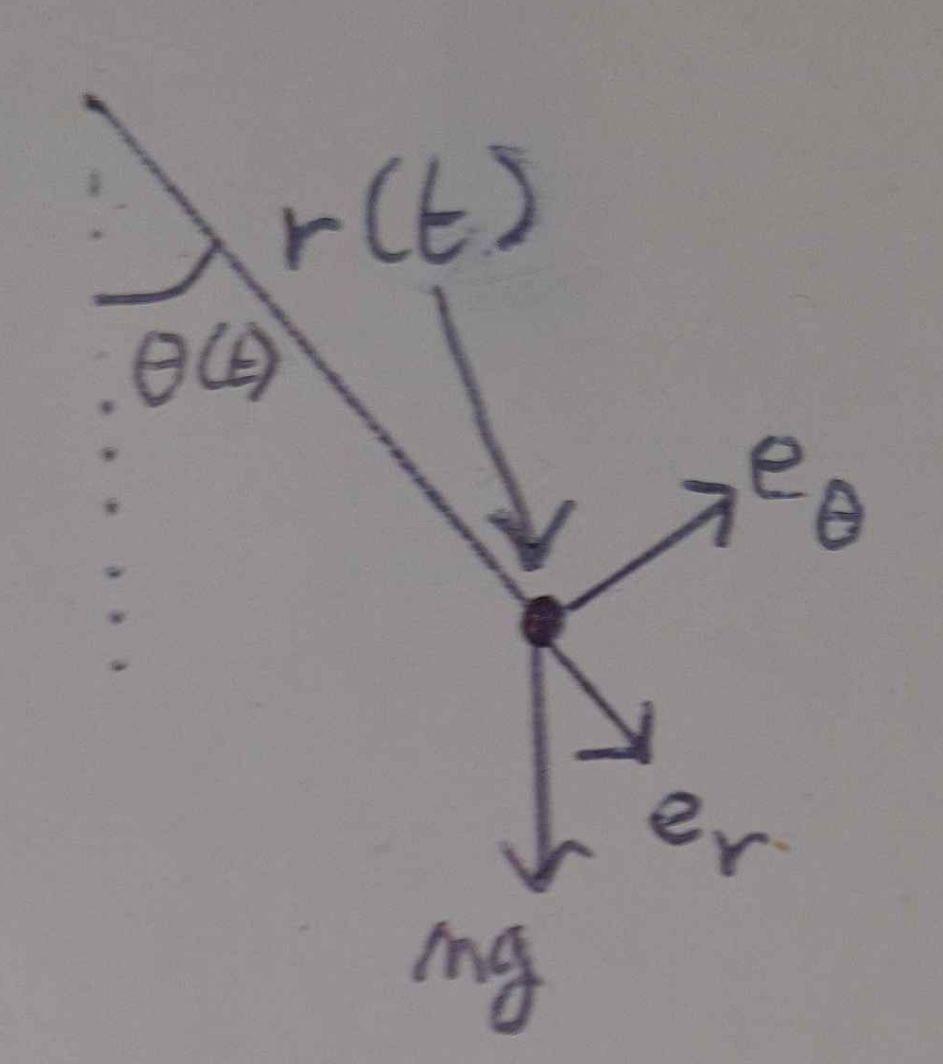
\includegraphics[width=0.5\textwidth]{Figures/Swing.png}
    \caption{The position $r(t)$ of the swing at time $t$. $\theta(t)$ describes the angle that the swing makes with a vertical axis. $e_r$ and $r_\theta$ are the respective basis vectors and $mg$ is the weight of the swing.}
    \label{fig1}
\end{figure}

Using the usual dot notation to indicate a derivative with respect to time, we can also find that:

\begin{align}
    \dot{\mathbf{e_r}} &= \frac{d\theta}{dt} \frac{d}{d\theta}(\mathbf{e_r}),\\
    &= \dot{\theta}(-sin(\theta) \mathbf{e_x} + cos(\theta) \mathbf{e_y}),\\
    &= \dot{\theta}\mathbf{e_\theta},\\
    \dot{\mathbf{e_\theta}} &= \frac{d\theta}{dt} \frac{d}{d\theta}(\mathbf{e_\theta}),\\
    &= \dot{\theta} (-cos(\theta) \mathbf{e_x} - sin(\theta) \mathbf{e_y}),\\
    &= -\dot{\theta} \mathbf{e_r}
\end{align}

Newton's second law gives us that $F = ma$, where $F$ is the net force, $m$ is the mass, and $a$ is the acceleration. In the case of our swing we therefore have that:

$$F = m g \mathbf{e_x} - T \mathbf{e_r}.$$

Here, $m$ is the mass of the swing, $g$ is the acceleration due to gravity, and $T$ is the tension of the rope that attaches the swing to a fixed point. We can find the acceleration of the swing by taking two derivatives of it's position,

\begin{align}
    a &= \frac{d^2\mathbf{r}}{dt^2},\\
    &= \frac{d}{dt}(\frac{d}{dt}(r\mathbf{e_r})),\\
    &= \frac{d}{dt}(\dot{r} \mathbf{e_r} + r\mathbf{\dot{e_r}}),\\
    &= \frac{d}{dt}(\dot{r} \mathbf{e_r} + r\dot{\theta}\mathbf{e_\theta}),\\
    &= (\ddot{r} - r \dot{\theta}^2) \mathbf{e_r} + (2\dot{r} \dot{\theta} + r \ddot{\theta}) \mathbf{e_\theta}.
\end{align}

If we rewrite the $\mathbf{e_x}$ in $F$ in terms of $\mathbf{e_r}$ and $\mathbf{e_\theta}$, we then get that Newton's second law gives us:

$$mg(cos(\theta) \mathbf{e_r} - sin(\theta) \mathbf{e_\theta}) - T\mathbf{e_r} = [(\ddot{r} - r \dot{\theta}^2) \mathbf{e_r} + (2\dot{r} \dot{\theta} + r \ddot{\theta}) \mathbf{e_\theta}]m$$

Looking at the $\mathbf{e_r}$ and $\mathbf{e_\theta}$ components separately gives us two equations:

\begin{align}
    \ddot{r} - r \dot{\theta}^2 &= gcos(\theta) - \frac{T}{m},\label{ODE1}\\
    2\dot{r} \dot{\theta} + r \ddot{\theta} &= -gsin(\theta).\label{ODE2}
\end{align}

Note that the $r \dot{\theta}^2$ term is the centrifugal force and the $2 \dot{r}\dot{\theta}$ corresponds to a Coriolis term.  Solving the two coupled ordinary differential equations will allow us to describe the motion more accurately.



Looking at equation \ref{ODE2}, and multiplying both sides of the equation by $r$ allows us to rewrite \ref{ODE2} as:

$$\frac{d}{dt}(r^2 \dot{\theta}) = -grsin(\theta).$$

We can then integrate both sides of the equation about a small interval $-\epsilon$ to $\epsilon$ and take the limit as $\epsilon \to 0$, where we let $\dot{\theta} > 0$ in the interval and choose $\epsilon$ to be $\ll 1$. This gives that the $RHS = 0$,
% I DONT REMEMBER WHY WE NEED TO ASK
and we are left with,

$$\lim_{\epsilon \to 0} \int_{-\epsilon} ^ \epsilon \frac{d}{dt}(r^2 \dot{\theta}) = 0.$$

Which implies that:

\begin{equation}
\lim_{\epsilon \to 0}\big[r^2 \dot{\theta}\big]^\epsilon_{-\epsilon} = 0,\label{Thetaeq}
\end{equation}

and therefore we can find the relationship between $\dot{\theta_-}$ and $\dot{\theta}_+$, the $\dot{\theta}$ evaluated at $t=-\epsilon$ and $t = \epsilon$ respectively. \ref{Thetaeq} implies:

$$\lim_{\epsilon \to 0}(r^2_{min} \dot{\theta} \big|_{t= -\epsilon} - r^2_{max} \dot{\theta} \big|_{t=\epsilon}) = 0$$

and so,

\begin{align}
    r^2_{min} \dot{\theta_-} - r^2_{max} \dot{\theta_+} = 0\\
    \implies \dot{\theta_+} = \frac{r^2_{min}}{r^2_{max}}\dot{\theta_-}
\end{align}

%i dont like my explanation here-JS

% i wasnt really sure what to write for our assumptions for why we put the heaviside in - JS

%-JS

\section{Limitations of the Model}
%limitations - e.g. valid for certain angles, works for solid steel swing pole, etc. -L

\section{Conclusion}
%conclusion, futher improvement suggestions - if improvements can be implemented quick and dirty may be worth as a subsection to the limitaitons section. -L


\section{Individual contributions}
\begin{itemize}
    \item Ben Crossland - contributions
    \item Chin Phin Ong (Linus) - Introduction and literary research
    \item Gabriella Iuliano - Conclusion
    \item Jacob Smith - Model
    \item Zayn Khan -
\end{itemize}

\newpage
\bibliographystyle{plain}
\bibliography{references}

\end{document}
